%!TEX root = ../report.tex

\begin{document}
    \chapter{基础功能}

    \section{顶点变换}
    \begin{spacing}{2.5}
    在软光栅渲染器中,顶点变换的基本任务是把空间三维顶点转换成屏幕上的二维坐标。这个过程涉及坐标变换的流水线,如图所示:\\
    \begin{figure}[H]
		\centering
		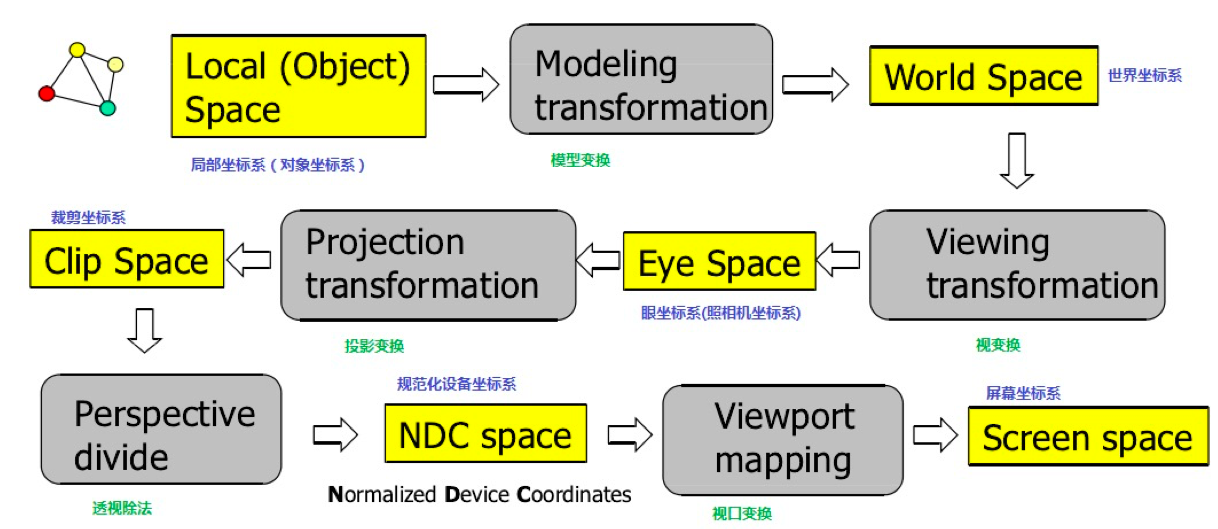
\includegraphics[width=1.0\textwidth]{images/pipline.png}
		\caption{软光栅渲染器坐标处理流水线}
		\label{line}
		\end{figure}
    \end{spacing}

    为了充分理解流水线各段,需要对几个坐标系进行理解。
    \subsection{局部坐标系}
    \begin{spacing}{2.5}
    每个物体在被创建时,都会有自己的局部坐标系,一般是以物体的几何中心为原点,那么物体的每个顶点相对于几何中心都会有一个相对坐标。这个坐标系就被称为物体的局部坐标系(Local Object Space)	
    \end{spacing}

    \section{裁剪}
    \section{线框画线}
\end{document}
